\clearpage
\section{Services}
\label{sec:builder-feature-services}

A service is what the public sees on the organization's portal, such as “Certificate request” or “Book an appointment”. Each service holds one or more forms and decides how it is delivered and who may apply. So a form reaches applicants only through a service; a form that belongs to no service stays an “internal form” for staff only.

\textbf{Path and who uses it:} “Builder” → “Core” → “Services”. Used by those who manage the organization's public services.

\begin{rcnote}[Example: Horizon]
Horizon accepts maintenance requests from its Aleppo customers, so the system administrator creates a “Maintenance request” service that starts with a published form and makes it available to registered accounts only. The “Branch visit request” form stays an internal form. They start the service from ①, and the visit form stays in ④.
\end{rcnote}

\begin{figure}[H]
\centering
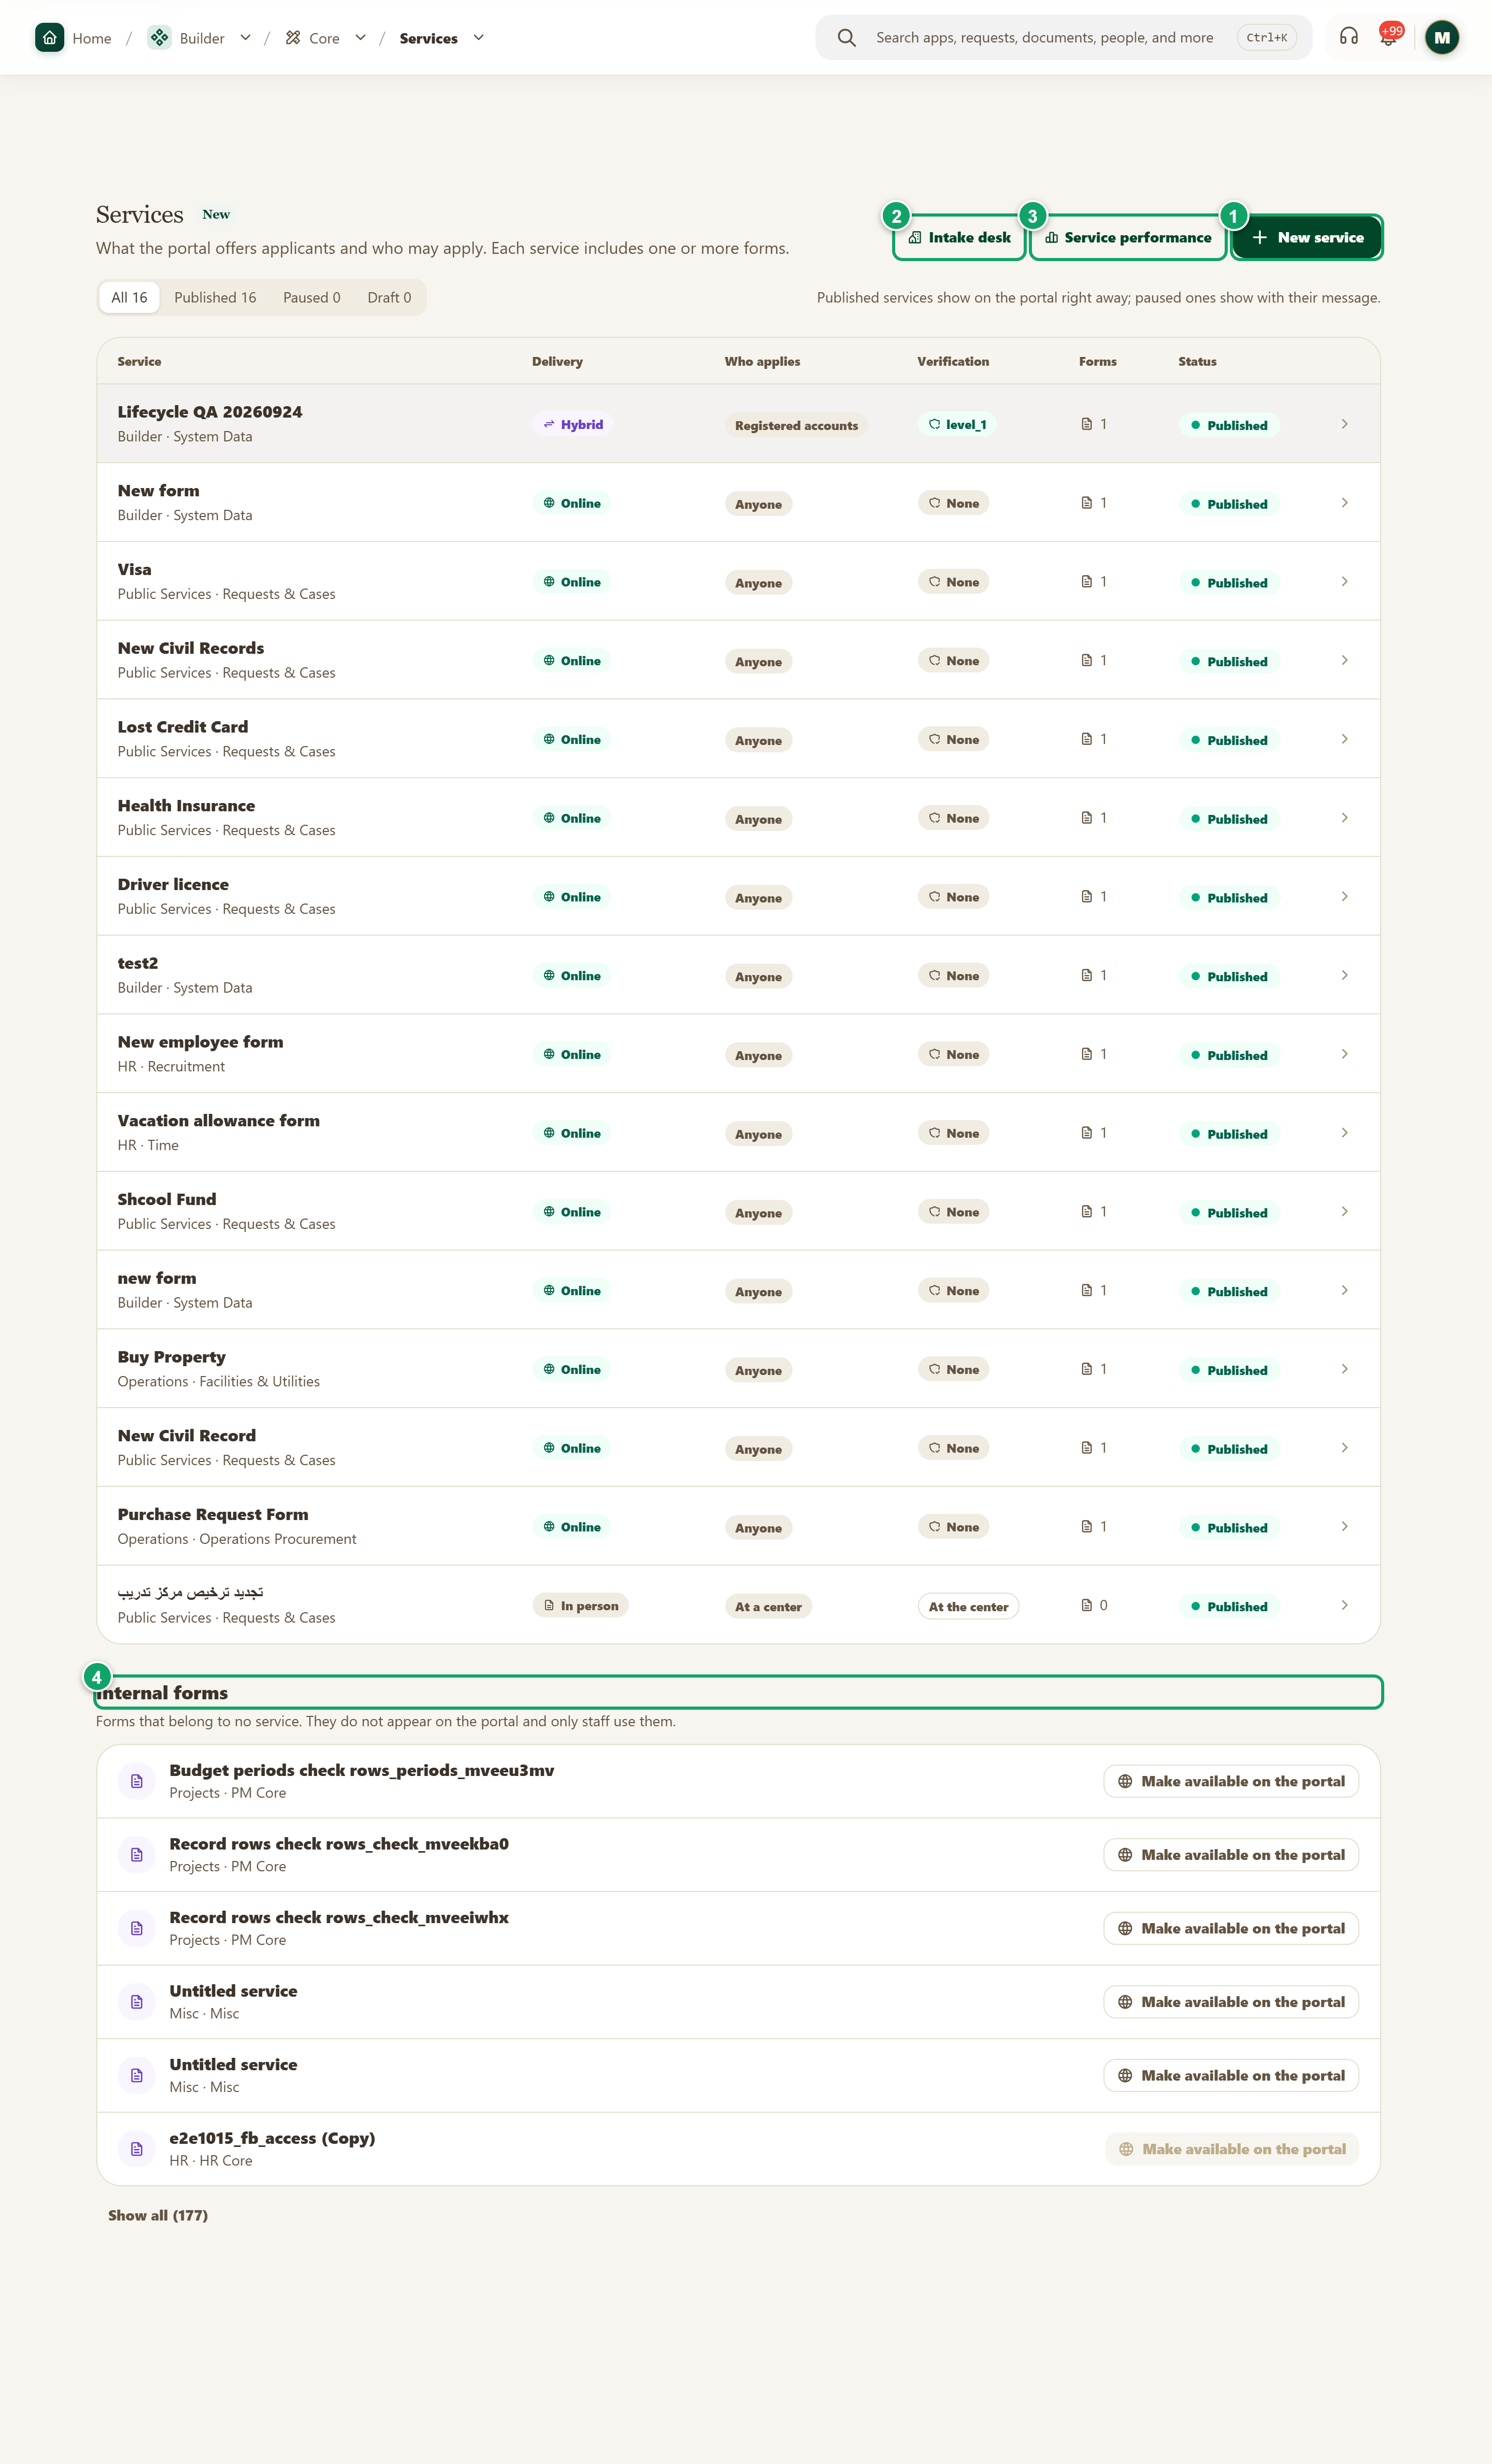
\includegraphics[width=0.95\linewidth,height=0.72\textheight,keepaspectratio]{figures/screens/ch06-services-en.png}
\caption{The “Services” page}
\label{fig:builder-services-screen}
\shotnote{The page lists the services shown on the portal and their state, then the internal forms that belong to no service. ① “New service”: starts a service around a published form. ② “Intake desk”: registers an in-person request. ③ “Service performance”: shows how requests move. ④ “Internal forms”: forms the public does not see.}
\end{figure}


\begin{table}[H]
\centering
\caption{What do you find here?}
\label{tab:builder-services-data}
\begin{tabularx}{\linewidth}{R{3.6cm} Y}
\rcHeaderRow
\thh{Part} & \thh{Content and action}\\
Services & The services table with “Delivery”, “Who applies”, “Verification”, forms and status, filtered by “Published”, “Paused” or “Draft”.\\
New service & Asks for the service name and the “Form the applicant starts with”, plus an optional staff record form.\\
Internal forms & Forms that belong to no service. “Make available on the portal” turns a published form into a new service or a step in an existing one.\\
Service page & Tabs “Overview”, “Fees”, “Profile”, “Delivery \& eligibility” and “Path \& forms”.\\
Intake desk and Service performance & Register an in-person request at a service center, and follow how requests move and where they wait.\\
\end{tabularx}
\end{table}

\begin{figure}[H]
\centering
\begin{tikzpicture}[node distance=0.5cm]
\node[entity] (service) {Service};
\node[entity,below right=0.7cm and 0.3cm of service] (entry) {Starting form};
\node[entityOpt,below left=0.7cm and 0.3cm of service] (more) {Path and follow-up forms};
\draw[dependsOn] (service.south) -- ++(0,-0.3) -| (entry.north);
\draw[dependsOnOpt] (service.south) -- ++(0,-0.3) -| (more.north);
\end{tikzpicture}
\rclegend
\caption{What a service holds}
\label{fig:builder-services-model}
\shotnote{The figure shows that a service needs a published starting form the applicant fills in, while the other forms are optional, such as later path steps or a follow-up form requested at a given status. So publish the form in the form builder first, then build the service around it.}
\end{figure}

\subsection{Steps and check}
\begin{enumerate}
\item Publish the form the applicant will start with on the “Forms” page.
\item Open “Services”, press “New service”, choose the form, then press “Create service”.
\item Complete the “Profile” the applicant reads, and set who may apply under “Delivery \& eligibility”.
\item Publish the service, then press “View on portal” to see it as the applicant does.
\end{enumerate}

\textbf{Check and recovery:} a published service should appear on the portal right away. If it does not, make sure it is not a “Draft”, because “Drafts are not on the portal”. To stop requests for a while, set it to “Paused” with a message to applicants instead of deleting it.
